\documentclass[12pt]{article}

%margó méretek
\usepackage[a4paper,
inner = 35mm,
outer = 25mm,
top = 25mm,
bottom = 25mm]{geometry}


%packagek, ha használni akarunk valamit menet közben
\usepackage{lmodern}
\usepackage[magyar]{babel}
\usepackage[utf8]{inputenc}
\usepackage[T1]{fontenc}
\usepackage[hidelinks]{hyperref}
\usepackage{graphicx}
\usepackage{amssymb}
\usepackage{epstopdf}
\usepackage{setspace}
\usepackage[nottoc,numbib]{tocbibind}
\usepackage{setspace}
\usepackage{wrapfig}
\usepackage{float}
\usepackage{blindtext}
\usepackage{enumitem}
\usepackage{amsmath,amssymb}
\usepackage{relsize}
\usepackage{listings}
\usepackage{color}
\usepackage{upquote}

\lstdefinelanguage{FSharp}%
{morekeywords={let, new, match, with, rec, open, module, namespace, type, of, member, % 
and, for, while, true, false, in, do, begin, end, fun, function, return, yield, try, %
mutable, if, then, else, cloud, async, static, use, abstract, interface, inherit, finally, private },
 otherkeywords={ let!, return!, do!, yield!, use!, var, from, select, where, order, by },
 keywordstyle=\color{bluekeywords},
 % new keyword colors
 classoffset=1,
 morekeywords={int, string, List, GCD, Tick, Rotation, BuffType, Condition, Buff, float, Map, bool, list, option, Skill, Combo, Job, Buff, ActionType, CooldownType, CostType, CastType, SkillType},
 keywordstyle=\color{cyantypes},
 classoffset=0,
 sensitive=true,
 basicstyle=\ttfamily,
   breaklines=true,
 xleftmargin=\parindent,
 aboveskip=\bigskipamount,
   tabsize=4,
 morecomment=[l][\color{greencomments}]{///},
 morecomment=[l][\color{greencomments}]{//},
 morecomment=[s][\color{greencomments}]{{(*}{*)}},
 morestring=[b]",
 showstringspaces=false,
 literate={`}{\`}1,
 stringstyle=\color{redstrings},
}

\definecolor{dkgreen}{rgb}{0,0.6,0}
\definecolor{gray}{rgb}{0.5,0.5,0.5}
\definecolor{mauve}{rgb}{0.58,0,0.82}
\definecolor{cyantypes}{rgb}{0.18,0.56,0.72}

\lstset{frame=tb,
  language=fsharp,
  aboveskip=3mm,
  belowskip=3mm,
  showstringspaces=false,
  columns=flexible,
  basicstyle={\small\ttfamily},
  numbers=none,
  numberstyle=\tiny\color{gray},
  keywordstyle=\color{blue},
  commentstyle=\color{dkgreen},
  stringstyle=\color{mauve},
  breaklines=true,
  breakatwhitespace=true,
  tabsize=3
}

\setstretch{1.5}
\begin{document}

\begin{titlepage}
	\vspace*{0cm}
	\centering
	\begin{tabular}{cp{1cm}c}
		\begin{minipage}{4cm}
			\vspace{0pt}
			
\includegraphics[width=1\textwidth]{elte_cimer}
		\end{minipage} & &
		\begin{minipage}{7cm}
			\vspace{0pt}Eötvös Loránd Tudományegyetem \vspace{10pt} \newline
			Informatikai Kar \vspace{10pt} \newline
			Komputeralgebra Tanszék
		\end{minipage}
	\end{tabular}
	
	\vspace*{0.2cm}
	\rule{\textwidth}{1pt}
	
	\vspace*{4cm}
	{\Huge Gépi tanulás a legynagyobb sebzés eléréséhez }
	
	\vspace*{9cm}
	
	\begin{tabular}{cp{1cm}c}
		\begin{minipage}{7cm}
			\vspace{0pt}Dr. Vatai Emil \vspace{10pt} \newline
			Adjunktus \newline
			Komputeralgebra tanszék \newline
			ELTE IK
		\end{minipage} & &
		\begin{minipage}{7cm}
			\vspace{0pt}Szalóki Sándor \vspace{10pt} \newline
			Programtervező informatikus BSc.
		\end{minipage}
	\end{tabular}
		
	
	\vfill
	
	\vspace*{1cm}
	Budapest, 2018
\end{titlepage}

\tableofcontents
\newpage

\section{Bevezető}

Legfőbb célom a szakdolgozattal a gépi tanulás mélyebb megértése, tanulása egy olyan példán keresztül, amely előfordulhat problémaként a való életben is.
\newline
A probléma, amivel itt foglalkozunk kellően bonyolult ahhoz, hogy a megoldásához gépi tanulást kelljen alkalmazni és megoldása ne legyen triviális egy egyszerű algoritmussal.
\newline
Ahhoz, hogy a feladat több legyen, mint egy egyszerű út keresés, minden lépés hatással van a környezetére, illetve a környezettől függően egy-egy lépés hatása, értéke változhat.
\newline
Erre egy kellő nehézségű probléma a Final Fantasy XIV harcrendszerének szimulálása, majd ebben a szimulációban való tanulás.

\pagebreak

\section{Felhasználói dokumentáció}

\subsection{Feladat}

\subsubsection{Játék modell}

Első feladat a játéknak egy kellő pontosságú modellezése. A megoldás hatékonysága érdekében törekedni kell arra, hogy ne legyen felesleges adat, viszont minden, ami szükséges, az elérhető legyen. 
A harcrendszer szabályai pontosan meghatározhatóak, így a szimulációtól elvárható a pontos eredmény is. 
Két fő részre osztható a modell: Karakterek és ezek képességei.

\paragraph{Karakterek}

Minden karakternek három meghatározó eleme van:

\begin{description}[align=right,labelwidth=3cm]
	\item [Gyorsaság] Ez adja meg a karakter globális időzítőjét
	\item [Támadás] A képesség, ami a játékos irányítása nélkül történik a karakter gyorsaságától függően
	\item [MP/TP] Magic Points, illetve Tactial Points, ezek a képességek erőforrásai
\end{description}

\paragraph{Képességek}

Egy képesség leírásához hét tulajdonság szükséges:

\begin{description}[align=right,labelwidth=3cm]
	\item [Potenciál] A sebzés mértékének alapja
	\item [Időzítő] Meghatározza, hogy az adott képesség a globális időzítőt, vagy a sajátját használja
	\item [Erőforrás] A használatának ára MP, vagy TP-ben
	\item [Combo] Képességek adott sorrendben használata esetén más-más lehet egy képesség hatása
	\item [Típus] Fegyver, vagy varázslat
	\item [Feltétel] A használatára vonatkozó feltétel
	\item [Hatás] Használat után adott ideig hatással lehet a következő képességere, a hős állapotára, vagy adott időközönként plusz sebzést okozhat
\end{description}

A karakter tulajdonságai és képességeinek listája alapján egy adott képesség sorozatból készíthető egy szimuláció, amely megadja, hogy a sorozatot hány tizedmásodperc végrehajtani, illetve végrehajtás után ennek mekkora a teljes sebzési értéke.
\newline
Fontos, hogy a szimuláció bármely pontján tudjuk, hogy mi a játékos pontos állapota: Erőforrásainak, globális időzítőjének, képességeinak saját időzítőjének állapota, az aktív hatások, illetve ha van, akkor a Combo álltal meghatározott következő képesség.
\newline
Ez az állapot megfelel annak, amit a játékos játék közben a képernyőn láthatna.

\subsubsection{Gépi tanulás}

A feladat ebben a szimulációban egy olyan képesség sorozat keresése, amely eléri a felhasználó álltal megadott időt, és ezalatt az idő alatt minél hatékonyabb legyen, azaz a legnagyobb sebzés elérésére törekszik.
\newline
A probléma tér elég nagy ahhoz, hogy egy egyszerű kereső algoritmus futási ideje túl nagy legyen. Ennek megoldásához megerősítéses tanulást használ a program.
\newline
Ehhez szükséges, hogy a játék állapotáról egy kellően pontos képet kapjunk, erre szolgál a játék szimulációjából tudható képszerű adat. Ezt az adatot állapotnak, a képességeket pedig akcióknak használhatjuk fel.

\subsubsection{Grafikus felület}

Szükséges egy egyszerű grafikus felület, amely megkönnyíti a program használatát, átláthatóságát. A képességek sorozatának egy megjelenítését, a gépi tanulás eredményének grafikus feldolgozását.
\newline
Az algoritmus eredményessége jól bemutatható néhány egyszerű grafikonon.

\pagebreak

\subsection{Módszerek}

A feladat megoldása funkcionális programozással történik.

\subsubsection{Játék model}

Az említett két fő elemet (Karakterek és Képességek) megfelelő típusokkal felvesszük, majd egy-egy tetszőleges karaktert a képességeivel együtt már egyszerűen előállíthatunk.
Miután kellő adat birtokában vagyunk, a képességekből összeállíthatunk egy sorozatot, amit szimulálni szeretnénk.
\newline
A játék harcrendszerének szimulációja három lépésben történik.
\begin{enumerate}
	\item A képességek sorozatát validálni kell. Ellenőrizni kell, hogy a képesség időzítője szerint lehetséges-e már a használata, rendelkezésre áll-e megfelelő típusú és mennyiségú erőforrás. Illetve néhány képesség rendelkezhet saját feltétellel, amit szintén ellenőrizni kell. Amennyiben minden rendelkezésre áll, a képességet meg kell tartani és a megfelelő hatásokat, illetve időzítőket be kell állítani.
	\item A validált sorozaton végig kell menni és minden ponton az adott állapot szerint ki kell számolni, hogy abban a tizedmásodpercen mennyi sebzés történt, majd ezeket összegezni.
\end{enumerate}

\subsubsection{Gépi tanulás}

A megfelelő algoritmus választásához több tényezőt is figyelembe kell venni. A játék harcrendszerének teljes működése kellően bonyolult, így a működést kihasználó algoritmusok használata bonyolult, ha lehetséges. 
Az akciók értéke az állapottól függ, illetve az akciók változtathatják az állapotot, emiatt az a feladat nem vezethető vissza egy egyszerű többkarú rabló problémára sem.
\newline
A probléma megoldásához Monte-Carlo-módszer használható. Az algoritmusnak nincs szüksége a háttérben működő szimuláció pontos leírására, elég ha tudunk adni egy pontos képet az állapotról, illetve az adott állapotban választott akciók értékéről.
\newline
A szimulációt olyan módon működik, hogy megfelelő képet tudjon adni az állapotról, az akció értéke pedig megadható az képesség sebzésének függvényében.

\subsubsection{Grafikus felület}

A program nem igényel bonyolult grafikus felületet. Egyszerű MVVM architektúra használatával épül fel WPF segítségével. 
Karaketerenként a kilistázzuk a képességek képeit, amelyek majd választhatóak lesznek szimulációra. Lehetőséget kell adni az eredmény sorozatnak kilistázására, illetve grafikonok rajzolására.
Fontos, hogy a számolás a háttérben fusson, hiszen ez egy idő után nagy számításokkal járhat, ami zárolhatja az ablakot.

\subsection{Rendszer-követelmények, telepítés}

A program futtatásához Windows operációs rendszer szükséges. Telepítés nem szükséges, viszont a futtatható állomány mellé el kell helyezni a (programmal együtt kiadott) dinamikus könyvtárakat is.

\paragraph{Ajánlott hardware:} 

Quad-Core 2.3 Ghz processzor, 2 GB RAM

\paragraph{Software követelmény:} 

Microsoft .NET Framework 4.6.1

\pagebreak

\subsection{A program használata}

A program indításához a futtatható állomány szükséges. Ennek indításával rögtön egy ablak fogad (\ref{fig:start}). Az ablakon található egy menüsor rendre Add, Start, illetve Cancel gombokkal. Alatta található a program futásához szükséges beállítások mezői. Egy listában találhatóak a karakterek és hozzájuk rendelt képességek listája. Az ablak közepén kerül majd megjelenítésre a tanult képesség sorozat, majd alatta a két grafikon. Továbbá található még egy státusz sor a képernyő legalján. Ebben a következő információk találhatóak: 

\begin{description}[align=right,labelwidth=3cm]
	\item [Status] Rövid üzenet a program állapotáról
	\item [Generations] A jelenlegi generáció száma
	\item [Damage] A tanult képesség sorozat álltal elért sebzés értéke
	\item [Duration] A tanult képesség sorozat álltal elért idő tizedmásodpercben
	\item [Bar] Töltő csík, amely mutatja, ha éppen számolás történik a háttérben
\end{description}

\begin{figure}[H]
	\begin{center}
		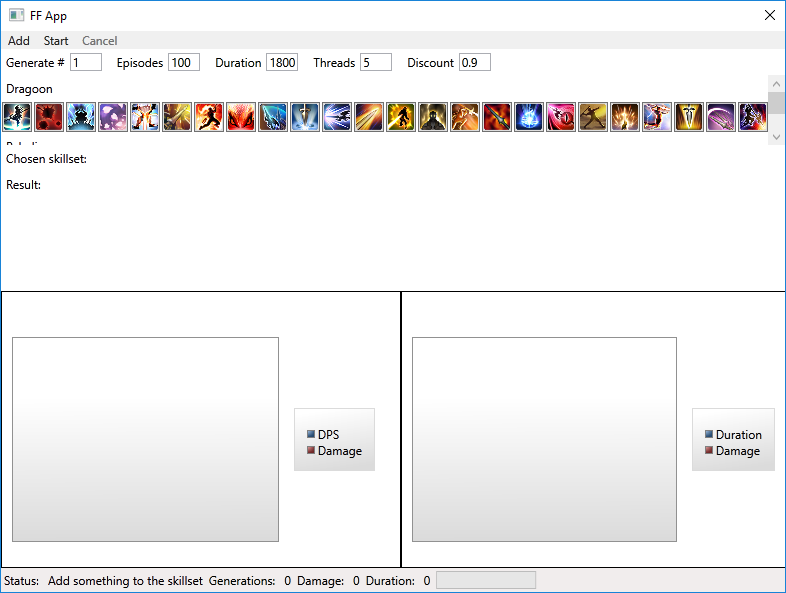
\includegraphics[width=1\textwidth]{start}
	\end{center}
	\caption{Kezdő képernyő}
	\label{fig:start}
\end{figure}

Mielőtt elindíthatnánk a tanulást, választanunk kell egyet a megadott karakterek képességlistái közül (\ref{fig:skilllist}). Minden képesség lista fölött megtalálható a hozzá tartozó karakter neve. A kurzor egy képességen tartása után megjelenik a képesség neve, rövid leírása. 

\begin{figure}[H]
	\begin{center}
		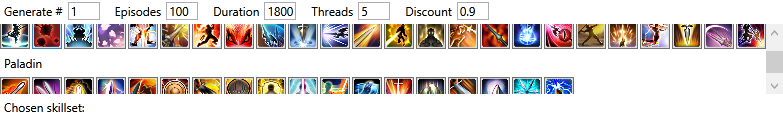
\includegraphics[width=1\textwidth]{skilllist}
	\end{center}
	\caption{Lehetséges választható listák}
	\label{fig:skilllist}
\end{figure}

Ha megtaláltuk a megfelelő listát, akkor az Add menüpontban (\ref{fig:addmenu}) választhatjuk ki a szükséges listát név alapján. Fontos, hogy ilyenkor még szabadon cserélhetjük a karaktert, ez a menüpont Start-ra kattintás után nem lesz előrhető. (Kivéve a New gomb)

\begin{figure}[H]
	\begin{center}
		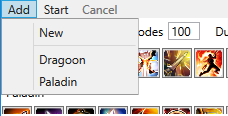
\includegraphics[width=0.4\textwidth]{addmenu}
	\end{center}
	\caption{Lehetséges választható listák az Add menüpont alatt}
	\label{fig:addmenu}
\end{figure}

A lista kiválasztása után erről információt kapunk, a választott lista megjelenik a Chosen skillset alatt (\ref{fig:chosen}). Ezen a ponton a tanulás elindítható a Start gombbal.

\begin{figure}[H]
	\begin{center}
		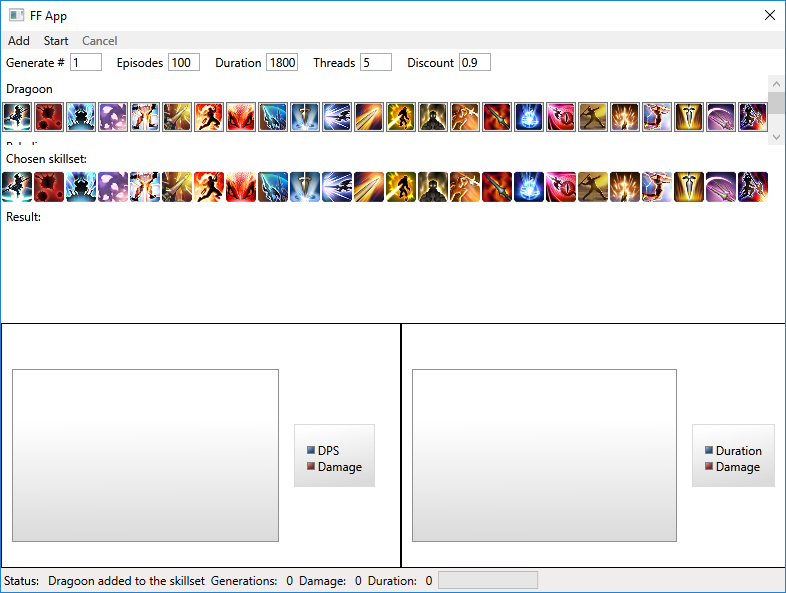
\includegraphics[width=1\textwidth]{chosen}
	\end{center}
	\caption{A választott lista megjelenik a képernyőn}
	\label{fig:chosen}
\end{figure}

Indítás előtt lehetőségünk van néhány beállítás változtatására (\ref{fig:options}).

\begin{figure}[H]
	\begin{center}
		
\includegraphics[width=0.7\textwidth]{options}
	\end{center}
	\caption{Futási beállítások}
	\label{fig:options}
\end{figure}

A beállítások sorra:

\begin{description}[align=right,labelwidth=3cm]
	 \item [Generate] A kívánt generációk számát adhatjuk meg
	 \item [Episodes] Generációnként létrehozott szimulációk száma
	 \item [Duration] Szimulációk hossza tizedmásodpercben
	 \item [Threads] Párhuzamosítás során használható magok száma
\end{description}

Amennyiben a beállításokat megfelelőnek találjuk, a Start gomb (\ref{fig:startgen}) lenyomásával elindítható a beállított számú generációk generálása. 

\begin{figure}[H]
	\begin{center}
		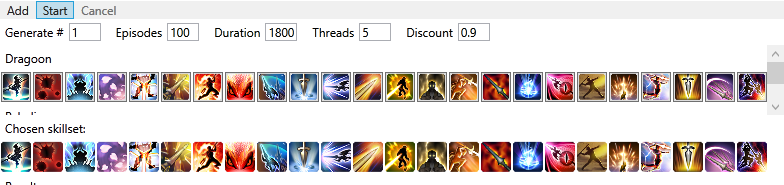
\includegraphics[width=1\textwidth]{startgen}
	\end{center}
	\caption{Generálások indítása}
	\label{fig:startgen}
\end{figure}

A program a generációkat egyesével állítja elő és rajzolja őket ki a képre (\ref{fig:15gen}). Eközben a beállítási mezők, illetve az Add és Start gombok nem elérhetőek, viszont a generálás bármikor leállítható a Cancel gombra kattintva.
Leállítást kérése esetén az éppen futó számolás még befejeződik, ennek eredménye megjelenik a képernyőn, majd az eddig letiltott mezők, gombok feloldásra kerülnek.

\begin{figure}[H]
	\begin{center}
		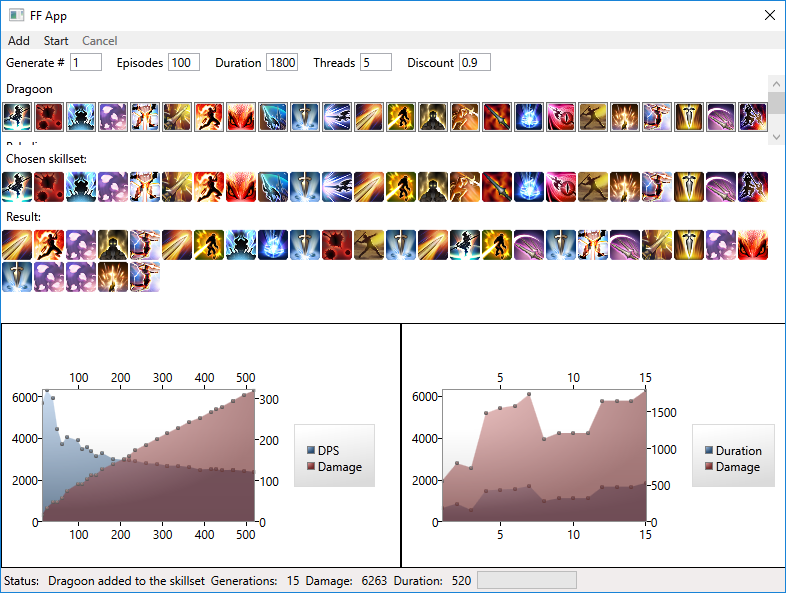
\includegraphics[width=1\textwidth]{15gen}
	\end{center}
	\caption{Eredmény 15 generáció futtatása után}
	\label{fig:15gen}
\end{figure}

Az eredményről három féle információt kapunk. 

\begin{description}[align=left,labelwidth=3cm]
	\item [Result] A jelenlegi tudás alapján generált képesség sorozat
	\item [Bal grafikon] A Result-ban szereplő képesség sorozat szimulálása során kapott sebzés értékek másodpercre osztott értékei. Kék színnel és Damage névvel jelölt terület mutatja az adott másodpercben elért teljes sebzést. Piros színnel és DPS névvel jelölt terület mutatja az adott másodpercben elért sebzés és idő hányadosát.
	\item [Jobb grafikon] Nyomon követhetjük minden generáció tudásának sebzés értékét
\end{description}

Amennyiben újra szeretnénk kezdeni a tanulás folyamatát, az Add menüpont alatt (\ref{fig:addmenu}) található egy New gomb, amivel alaphelyzetre állíthatjuk a programot. Ilyenkor a kiválasztott képesség lista nem változik, ennek változtatásához a programot újra kell indítani.

\section{Fejlesztői dokumentáció}

\subsection{Specifikáció}

A feladat egy karakter és annak képességeinek listájából létrehozni a legnagyobb sebzés értékű képesség sorozatot. A megfelelő specifikáció és az egyszerűség érdekében az alábbi két típust vezetjük be a játék modelljéből:

\vspace{1.5em}
\noindent\fbox{
	\begin{minipage}{\textwidth}
		$\mathcal{K} :$ Képesség

		$\mathcal{H} :$ Karakter
	\end{minipage}
}
\vspace{1em}

Ezek segítségével már megfogalmazhatóak a programra a következő állítások:

\vspace{1cm}
\noindent\fbox{
	\begin{minipage}{\textwidth}
		A = $(\underset{Karakter}{\mathcal{H}} \times \underset{Képességek}{\mathcal{K}^*} \times \underset{Eredmény}{\mathcal{K}^*})$
	
		B = $(\underset{Karakter'}{\mathcal{H}} \times \underset{Képességek'}{\mathcal{K}^*})$

		Q = $(Karakter = Karakter' \wedge Képességek = Képességek')$

		R = $(Sebzés(Karakter', Eredmény) = \underset{ks \in \mathcal{P}(Képességek')}{argmax} Sebzés(Karakter', ks))$

		$\quad$Sebzés$ : \mathcal{H} \times \mathcal{K}^* \rightarrow \mathbb{N}$
	\end{minipage}
} \vspace{1em}

Az állapottér tartalmazza a karaktert és annak használható képességeit, illetve az eredményt. Paramétertérnek felvesszük a karakter és képességeinek listájának egy kezdő állapotát.
Előfeltételként lerögzítjük a karakter és képességeinek listájának értékét.
Utófeltétel, hogy az eredmény álltal meghatározott képesség sorozat sebzés értéke az adott karakterrel maximális. 
Ennek meghatározása a képességek számával arányosan exponenciálisan nő, ezért fontos egy olyan algoritmus használata, amely ezt hatékonyan képes kiszámolni.

\subsection{Módszerek}

\subsubsection{Játék model}

A játék modellezéséhez szükséges a két alaptípus: Karakter és Képesség. Ezeket egy-egy a leírásnak megfelelő típussal könnyen le is írhatjuk.

\paragraph{Skill}
A Skill típus reprezentálja a Képességet. Ennek a leírása a következő:

\pagebreak
\begin{lstlisting}
type Skill =
	{
		Name            : string
		Potency         : int
		Action          : ActionType
		CooldownType    : CooldownType
		CostType        : CostType
		CastType        : CastType
		SkillType       : SkillType
		Combo           : Combo list option
		Condition       : (Buff list -> bool) option
		ID              : int
	}
\end{lstlisting}

Ahhoz, hogy a képesség modellje elég pontos legyen a játék szimulációjához, az alabbi típusokkal jellemezzük a tulajdonságait:

\begin{lstlisting}
type CooldownType =
| GlobalCooldown
| OffGlobalCooldown of int

type CostType =
| Free
| MP of int
| TP of int

type CastType =
| Instant
| Time of int

type SkillType =
| Ability
| Weaponskill
| Spell

type ActionType = 
| Damage of Buff list option
| DamageOverTime of potency:int * duration:int * Buff option
| Buff of Buff list
| Debuff of Buff
| Heal of Buff option
and BuffType =
| Job of (Job -> Job)
| Skill of (Skill -> Skill)
| BuffDuration of (Buff -> (Buff * int * int) option)
and Buff =
{
	Name        : string
	Effect      : BuffType
	Duration    : int
	Condition   : Condition
	Stacks      : int
	EndEffect   : (Buff -> Buff) option
	ID          : int
}
and Condition =
| NotLimited
| LimitedUses of uses:int * contidion:(Skill * Job * Buff list -> bool)
and Combo =
{
	Name            : string
	Target          : string
	Effect          : Skill -> Skill
	DistruptedByGCD : bool
	NotFirst        : bool
}
\end{lstlisting}

\pagebreak
\paragraph{Job}
A Job típus valósítja meg a karaktert. Ennek jellemzése hasonló módon történik. Tulajdonságai jól megfeleltethetőek egy-egy típusnak:

\begin{lstlisting}
type Job =
{
	Name        : string
	Speed       : int
	AutoAttack  : Skill
	MaxMP       : int
	MP          : int
	TP          : int
}
\end{lstlisting}

\paragraph{Rotation}

Ezek segítségével a szimulációt reprezentáló típust nehézéges nélkül hozhatjuk létre a következő módon:

\begin{lstlisting}
type GCD =
| Cooldown of int
| Available

type Tick =
{
	ActiveBuffs         : (Buff * int) list
	ActiveDebuffs       : (Buff * int) list
	OGCDTimers          : (Skill * int) list
	GCDtick             : GCD
	ActiveSkill         : Skill option
	ActiveDoTs          : (Skill * (int * int)) list
	ActiveCombo         : (Combo list * int) option
}

type Rotation = 
| Rotation of (Tick list) * Job
\end{lstlisting}

\pagebreak

A képesség sorozat végleges szimulációja a Rotation típusban jelenik meg. Az ebben szereplő Tick lista reprezentálja az idővonalat, egy Tick egy tizedmásodpercet jelöl.
Ezzel a megoldással a szimuláció bármely pontján kérhetünk információt az adott tizedmásodperc adatairól. 
Tudjuk az éppen aktív pozitív, negatív hatásokat, minden képesség saját időzítőjét (amennyiben rendelkezik saját időzítővel), 
a globális időzítő állását, az éppen használt képességet (ha létezik), az aktív időszakos sebzéseket, illetve tudjuk, ha létezik éppen aktív combo (akár több is).

\paragraph{Szimuláció}

Ahhoz, hogy a Rotation Tick listájába adat kerüljön, szükséges egy függvény, amivel a szimulációhoz úgy adhatunk új képességeket, hogy az validálva legyen, illetve a lehető legnagyobb pontosággal tükrözze a való életben történő eseményeket.
Ezt a feladatot a Rotation Add függvénye végzi el. 

\begin{lstlisting}
static member add (skill: Skill) (rotation: Rotation) =
	match rotation with
	| Rotation (ticks, job) ->
		match ticks with
		| [] -> failwith "Failed to add skill to the rotation"
		| ticks ->
			let ticks = ticks |> List.indexed
			let lastindex, last = ticks |> List.last
			let job = Rotation.updateJob job lastindex last
			let orignalSkill = skill
		.
		.
		.
\end{lstlisting}

\subparagraph{Global Cooldown - GCD} 
Miután feloldottuk a típust és megszereztük az eddigi Tick listát, elkezdhetjük előállítani a következő Tick adatait.
Először megnézzük, hogy az előző állapotban mi volt a globális időzítő értéke és beállítjuk az állapota alapján az megfelelő értékre.

\subparagraph{Skill}
Következő lépésben az éppen használni kívánt képességet az aktív hatások és combo alapján frissítjük. Kihasználjuk, hogy a hatások típusa (Skill $\rightarrow$ Skill), így ezek kompozíciójával egyszerűen számolhatunk.

\subparagraph{Combo}
Miután az aktív képességet a hatások álltal meghatározott állapotára hoztuk, beállíthatjuk ez alapján az combo értékét is. Sok esetben egy képesség csak akkor kap combo tulajdonságot, ha már ő maga is az előző combo célja volt, ezért fontos, hogy ez a lépés a frissítés után történjen.
Amennyiben a képesség nem rendelkezik ilyen tulajdonsággal, az előző állapotot kell tovább vinnünk. Ha az előző állapotban megadott Combo időzítője lejárt, ezt törölni kell.

\subparagraph{Buff}
A Combo tulajdonsághoz hasonlóan a képességhez tartozó új hatások is más hatások eredménye képpen kerülhetnek csak elő. Ezeket a megfelelő időzítővel ellátva rakjuk bele hatások listájába.
Ezeken a listákon végig kell menni és ellenőrizni, hogy az időzítőjük alapján törölni kell-e őket. 

\subparagraph{Cast Time}
Fontos, hogy egy képesség használata mennyi időt vesz igénybe, hiszen e szerint kell használat után további "üres" Tick-ekkel feltölteni a szimulációt, amivel garantáljuk az idő múlását.

\subparagraph{Damage over Time - DoT}
Képességeknek lehetőségük van nem csak egyszeri sebzést okozni, de megadott ideig időközönkénti sebzést okozni. Ezeket az időközönkénti sebzéseket is külön tárolnunk kell egy listában.
A listát ellenőrizni kell, amennyiben egy időzítő lejárt, a hozzá tartozó elemet törölni kell.

\subparagraph{Off Global Cooldown - OGCD}
A saját időzítővel rendelkező képességek időzítőinek listáján is végig kell menni és a lejárt időzítőket törölni kell.

\subparagraph{Condition}
Képességeket az időzítőjük típusától függően különböző feltételekkel tehetjük csak be a szimulációba.
Közös működés történik amennyiben a képességhez szükséges erőforrás nem áll rendelkezésre (ekkor addig várunk, amíg megfelelő mennyiségű erőforrás keletkezik), illetve amikor a képesség saját feltétele (ha van) nem teljesül. Ha a saját feltétel nem teljesül, akkor a képesség használata nem szabályos, nem kerül be a szimulációba.

\begin{description}[align=right,labelwidth=3cm]
	\item [GCD] Az egyszerűbb eset, amikor a globális időzítőt használja a képesség. Ekkor megvárjuk a globális időzítő végét, majd a képességet hozzá adjuk a szimulációhoz és újra indítjuk a globális időzítőt.
	\item [OGCD] Ebben az esetben ellenőrizni kell, hogy a képesség saját időzítője már benne van-e az aktív időzítők listájában. Amennyiben benne van, a képességet nem tudjuk használni. Ellenkező esetben a képesség időzítőjét elindítjuk, a képességet hozzá adjuk a szimulációhoz.
\end{description}

\subparagraph{Üres Tick}
Sokszor van szükség "üres" időtöltésre, ekkor a szimulációt ugyan ezek a szabályok alapján, de aktív képesség nélkül töljük fel megfelelő számú új Tick-el.

\paragraph{Sebzés számlálás}

Miután a képesség sorozatból megkaptuk a megfelelő validált szimulációt, lehetőségünk van ezen végig menni és megszámolni a sorozat teljes sebzés értékét. A szimulált sorozatban minden képesség sebzés értéke már rendelkezik a hatások módosításaival, tehát ezt nem kell újra számolni. 
Minden karakter rendelkezik egy sebesség tulajdonsággal, illetve egy alapvető támadással, ezt itt kell nyomon követnünk. A sebesség álltal meghatározott időközönként ezt a támadást hozzá kell adnunk a szimulációban található sebzésekhez. Ez a támadás szintén élvezheti a hatások módosításait, tehát ezeket is itt kell hozzá adnunk az előbb használt módon.
Található még a szimulációban időközönkénti sebzés is, amit szintén itt kell nyomon követnünk.
\newline
Ebből a három tényezőből már egy számszerű sebzés érték rendelhető minden Tick-hez. Ezeket az értékeket összegezve megkapjuk a szimuláció teljes sebzési értékét.

\begin{lstlisting}
let ToDamage (rotation: Rotation) : int =
	match rotation with
	| Rotation (rotation, job) ->
		let time = (List.length rotation) / 10
		rotation
		|> List.indexed
		|> List.fold (fun dps (index, tick) ->
		.
		.
		.
\end{lstlisting}

\subsubsection{Gépi tanulás}

A választott algoritmus az Off-Policy Monte Carlo módszer az optimális $\pi \approx \pi_*$ stratégia eléréséhez.
\newline
Az eredeti algoritmus ehhez a következő: \vspace{1cm}

\noindent\fbox{
	\begin{minipage}{\textwidth}
		Kezdetben $\forall s \in \mathcal{S}: \forall a \in \mathcal{A}(s):$

		$\quad\mathnormal{Q}(s, a) \in \mathbb{R} \quad$ (tetszőleges)

		$\quad\mathnormal{C}(s, a) \leftarrow 0$

		$\quad\pi(s) \leftarrow argmax_a \mathnormal{Q}(s, a)$

		Végtelen ciklus (minden szimulációra) :

		$\quad b \leftarrow$ tetszőleges gyenge stratégia

		$\quad$Szimuláció léterehozása b-t használva: $\mathnormal{S}_0, \mathnormal{A}_0, \mathnormal{R}_1, ... , \mathnormal{S}_{T-1}, \mathnormal{A}_{T-1}, \mathnormal{R}_T$  

		$\quad\mathnormal{G} \leftarrow 0$

		$\quad\mathnormal{W} \leftarrow 1$

		$\quad$Ciklus a szimuláció minden lépésére, $t = \mathnormal{T} - 1, \mathnormal{T} - 2, ..., 0 :$

		$\quad\quad\mathnormal{G} \leftarrow \gamma\mathnormal{G} + \mathnormal{R}_{t+1}$

		$\quad\quad\mathnormal{C}(\mathnormal{S}_t,\mathnormal{A}_t) \leftarrow C(S_t,A_t) + W$

		$\quad\quad\mathnormal{Q}(S_t, A_t) \leftarrow Q(S_t, A_t) + \frac{W}{C(S_t, A_t)} [G - Q(S_t, A_t)]$

		$\quad\quad\pi(S_t) \leftarrow argmax_a Q(S_t, a)$

		$\quad\quad$Ha $A_t \neq \pi(S_t)$: Ciklus vége

		$\quad\quad\mathnormal{W} \leftarrow W\frac{1}{b(A_t|S_t)}$
	\end{minipage}
} \vspace{1.5em}

Mivel a program funkcionális nyelven készült, az algoritmust, ennek megfelelően kellett megváltoztatni.
Az algoritmus megvalósításához szükséges néhány változtatás. A használt típusok és függvények leírásai:

\vspace{1cm}
\noindent\fbox{
	\begin{minipage}{\textwidth}
		$\mathcal{S} : \mathbb{N}^* \times \mathbb{N}^* \times \mathbb{N}^* \times string^* \times \mathbb{N} \times \mathbb{N}$

		$\mathcal{A} : \mathbb{N}$

		$\mathcal{Q} : \mathcal{S} \times \mathcal{A} \rightarrow \mathbb{R}$

		$\mathcal{C} : \mathcal{S} \times \mathcal{A} \rightarrow \mathbb{R}$

		$\pi : \mathcal{S} \rightarrow \mathbb{R}^*$

		$\mathcal{E}: \mathcal{S} \times \mathcal{A} \times \mathbb{R}$

		Episode $: \mathcal{E}^*$
		
		GenerateEpisode $: \pi \rightarrow Episode$

		CreateRandomPolicy $: \pi$

		CreateGreedyPolicy $: \mathcal{Q} \rightarrow \pi$

		CreateEpsilonGreedyPolicy $: \mathcal{Q} \times \varepsilon \rightarrow \pi$

		MonteCarlo $: Q \times C \times \pi \rightarrow Q \times C \times \pi$
	\end{minipage}
}
\vspace{1.5em}

Ezek alapján az algoritmus megfeleltethető a következő függvénynek: 

\vspace{1cm}
\noindent\fbox{
	\begin{minipage}{\textwidth}
		MonteCarlo $: \mathcal{Q} \times \mathcal{C} \times \pi \rightarrow \mathcal{Q} \times \mathcal{C} \times \pi$

		MonteCarlo Q C b =

		$\quad$episodeFolder $: \mathbb{R} \times \mathcal{Q} \times \mathcal{C} \times \mathbb{R} \rightarrow \mathcal{E} \rightarrow \mathbb{R} \times \mathcal{Q} \times \mathcal{C} \times \mathbb{R}$

		$\quad$episodeFolder (G, Q, C, W) E =
		
		%$\quad\quad$(S, A, R) $: \mathcal{S} \times \mathcal{A} \times \mathbb{R}$

		$\quad\quad$(S, A, R) = E
		
		%$\quad\quad$g $: \mathbb{R}$
		
		$\quad\quad$g = $\gamma\mathnormal{G} + R$

		%$\quad\quad$c $: \mathcal{C}$
		
		$\quad\quad$c (S, A) = $C (S, A) + W$

		%$\quad\quad$q $: \mathcal{Q}$
		
		$\quad\quad$q (S, A) = $q (S, A) + \frac{W}{C (S, A)}[G - Q (S, A)]$

		%$\quad\quad$w $: \mathbb{R}$
		
		$\quad\quad$w = $W\frac{1}{b (S) | A}$

		$\quad\quad$(g, q, c, w)

		$\quad$episodes $: Episode^*$

		$\quad$episodes $= [$GenerateEpisode b$ | x \leftarrow [1..]]$
		
		$\quad$episodesFolder $: \mathcal{Q} \times \mathcal{C} \rightarrow Episode \rightarrow \mathcal{Q} \times \mathcal{C}$
		
		$\quad$episodesFolder (Q, C) E =

		%$\quad\quad$(g, q, c, w) $: \mathbb{R} \times \mathcal{Q} \times \mathcal{C} \times \mathbb{R}$
		
		$\quad\quad$(g, q, c, w) = foldl episodeFolder (0, Q, C, 1) E

		$\quad\quad$(q, c)

		%$\quad$(q, c) $: \mathcal{Q} \times \mathcal{C}$	
		
		$\quad$(q, c) = foldr episodesFolder (Q, C) episodes

		$\quad$q, c, CreateGreedyPolicy q

	\end{minipage}
}
\vspace{1.5 em}

Az itt található GenerateEpisode feladata az adott stratégia használatával létrehozni egy-egy szimulációt. Ehhez szükséges néhány új függvény a játék modell és a tanulás közötti átmenet miatt:

\vspace{1cm}
\noindent\fbox{
	\begin{minipage}{\textwidth}
		Random $: \mathbb{R}^* \rightarrow \mathbb{N}$

		ToSkill $: \mathbb{N} \rightarrow Skill$
		
		Add $: Skill \times Rotation \rightarrow Rotation$

		FromRotation $: Rotation \rightarrow \mathcal{S}$
		
		ToDamage $: Rotation \rightarrow \mathbb{N}$

		Time $: Rotation \rightarrow \mathbb{N}$

		EmptyRotation $: Rotation$

		Duration $: \mathbb{N}$
	\end{minipage}
}
\vspace{1.5 em}

Ezek használatával a szimuláció már egyszerűen létrehozható az alábbi módon:

\vspace{1cm}
\noindent\fbox{
	\begin{minipage}{\textwidth}
		GenerateEpisode $: \pi \rightarrow Episode$

		GenerateEpisode b = 
		
		$\quad$Generate $: Rotation \times \mathcal{S} \times \mathbb{L} \times Episode$

		$\quad$Generate Rot S l Ep =

		$\quad\quad$Ha l$: $ Ep

		$\quad\quad$A $: \mathcal{A}$

		$\quad\quad$A = Random (b S)
		
		$\quad\quad$(s, r, l, rot) $: \mathcal{S} \times \mathbb{R} \times \mathbb{L} \times Rotation$

		$\quad\quad$(s, r, l, rot) =

		$\quad\quad\quad$skill = ToSkill A

		$\quad\quad\quad$rotation = Add skill Rot

		$\quad\quad\quad$state = FromRotation rotation

		$\quad\quad\quad$reward = 

		$\quad\quad\quad\quad$Ha (Time Rot) = (Time rotation)$: $ -50
		
		$\quad\quad\quad\quad$Ha (Time rotation) > Duration$: $ 1000

		$\quad\quad\quad\quad$Különben$: \frac{ToDamage(rotation)}{Time(rotation)}$

		$\quad\quad\quad$finished = (Time Rot) = (Time rotation) $\vee$ (Time rotation) > Duration

		$\quad\quad\quad$(state, reward, finished, rotation)

		$\quad\quad$Generate rot s finished (Ep + (S, A, r))

		$\quad$Generate EmptyRotation (FromRotation EmptyRotation) False []
	\end{minipage}
}
\vspace{1.5 em}

\paragraph{Reward} 
Ezen a ponton szükséges minden állapothoz egy jutalom választása. A folyamatos magas sebzésre törekvés érdekében a jutalom az aktuális sebzés értéke és az eltelt idő hányadosa. Szükséges a rossz működés büntetése is. Amennyiben az akciót követően a szimuláció ideje nem változik, az adott akció egy nem megengedett akció volt. Ha a szimuláció időtartama eléri az előre megjelölt cél időt, a jutalom sokszorosát kapja.

\paragraph{Generációk}
A hatékonyság növelése érdekében a MonteCarlo $\pi$ értéke egy $\varepsilon$-mohó stratégia. További hatékonyság növelést érünk el, ha a generált szimulációk számát korlátozzuk, majd a tanult tudás alapján az algoritmust újra indítjuk úgy, hogy az új $\pi$-t ez alapján a tudás alapján hozzuk létre egy már kisebb $\varepsilon$ értékkel. Kezdetben az algoritmust egy igazságos véletlen szerű startégiával indítjuk el. Ezeket a meneteket hívjuk itt generációknak.

Egy generációs algoritmust ezek alapján a következő éppen fogalmazhatunk meg az eddig ismert típusok és függvények használata segítségével:

\vspace{1cm}
\noindent\fbox{
	\begin{minipage}{\textwidth}
		GeneticMonteCarlo $: \mathcal{Q} \times \mathcal{C} \times \pi \rightarrow \mathcal{Q} \times \mathcal{C} \times \pi$

		GeneticMonteCarlo Q C b =

		$\quad$Folder $: \mathcal{Q} \times \mathcal{C} \times \pi \rightarrow \mathbb{N} \rightarrow \mathcal{Q} \times \mathcal{C} \times \pi$
		
		$\quad$Folder (Q C b) i =

		$\quad\quad$epsilon = $\frac{1}{5 \times \ln{i + 5}}$

		$\quad\quad$(q, c, pi) = MonteCarlo Q C b

		$\quad\quad$(q, c, CreateEpsilonGreedyPolicy q epsilon)

		$\quad$(q, c, pi) = foldl Folder [1..] (Q, C, b)

		$\quad$q, c, CreateGreedyPolicy q
	\end{minipage}
}
\vspace{1.5 em}



\subsubsection{Grafikus felület}

\subsection{Szerkezet}

\subsubsection{Külső függőségek}

\subsubsection{Adatszerkezetek}

\subsubsection{Modulok}

\subsubsection{Képességek}

\subsection{Tesztelés}

\end{document}